\chapter{线性空间}

线性空间是线性代数的基本舞台。矩阵可以看作线性变换的坐标表示，线性方程组的解集常常构成一个线性空间，而模形式空间 $M_k(\Gamma)$ 在最基本的层面上也是复数域上的线性空间。本章从定义出发，系统讨论线性空间、线性相关与线性无关、基与维数、子空间与直和分解，以及商空间。读者应当特别熟悉“用基描述空间”和“用维数比较空间”这两种思想，因为它们会在后续各章反复出现。

\section{向量空间的定义与例子}

本章中，$\F$ 表示一个域。最常见的情形是 $\F=\R$ 或 $\F=\C$。

\begin{definition}
设 $V$ 是一个非空集合，其元素称为\emph{向量}；设 $\F$ 是一个域，其元素称为\emph{标量}。如果在 $V$ 上定义了加法
\[
+:V\times V\to V,\qquad (u,v)\mapsto u+v,
\]
以及数量乘法
\[
\F\times V\to V,\qquad (a,v)\mapsto av,
\]
并且对任意 $u,v,w\in V$ 与任意 $a,b\in\F$，下列公理都成立：
\begin{enumerate}[label=\textnormal{(\arabic*)}]
  \item $u+v=v+u$；
  \item $(u+v)+w=u+(v+w)$；
  \item 存在 $0\in V$，使得 $v+0=v$；
  \item 对每个 $v\in V$，存在 $-v\in V$，使得 $v+(-v)=0$；
  \item $a(u+v)=au+av$；
  \item $(a+b)v=av+bv$；
  \item $a(bv)=(ab)v$；
  \item $1v=v$，其中 $1$ 是域 $\F$ 的乘法单位元；
\end{enumerate}
则称 $V$ 是域 $\F$ 上的\emph{向量空间}（或\emph{线性空间}）。
\end{definition}

\begin{remark}
前四条公理说明 $(V,+)$ 是一个交换群；后四条公理说明数乘与域的加法、乘法相容。以后若未特别说明，所谓“向量空间”都指某个域上的向量空间。
\end{remark}

\begin{example}[欧氏空间]
$\R^n$ 在按分量加法与按分量数乘下是 $\R$ 上的向量空间：
\[
(x_1,\dots,x_n)+(y_1,\dots,y_n)=(x_1+y_1,\dots,x_n+y_n),
\]
\[
a(x_1,\dots,x_n)=(ax_1,\dots,ax_n).
\]
同理，$\C^n$ 是 $\C$ 上的向量空间。若把复数也只看成实数，则 $\C^n$ 还是 $\R$ 上的向量空间。
\end{example}

\begin{example}[多项式空间]
所有系数属于 $\F$ 的一元多项式构成集合 $\F[x]$。按通常的多项式加法和数乘，$\F[x]$ 是 $\F$ 上的向量空间。例如
\[
(a_0+a_1x+a_2x^2)+(b_0+b_1x+b_2x^2)=(a_0+b_0)+(a_1+b_1)x+(a_2+b_2)x^2.
\]
对每个非负整数 $d$，次数不超过 $d$ 的多项式集合
\[
\F[x]_{\le d}=\{f(x)\in\F[x]:\deg f\le d\}
\]
也是向量空间。
\end{example}

\begin{example}[函数空间]
设 $X$ 是非空集合。所有从 $X$ 到 $\F$ 的函数构成的集合记为
\[
\F^X=\{f:X\to\F\}.
\]
在逐点加法与逐点数乘下，$\F^X$ 是向量空间，即
\[
(f+g)(x)=f(x)+g(x),\qquad (af)(x)=a f(x).
\]
后面我们会把许多“函数满足某种线性条件的集合”看成 $\F^X$ 的子空间。
\end{example}

\begin{example}[矩阵空间]
$m\times n$ 矩阵全体 $\Mat_{m\times n}(\F)$ 在通常的矩阵加法与数乘下是向量空间。特别地，$\Mat_n(\F)$ 是 $n\times n$ 矩阵空间。
\end{example}

\begin{proposition}[齐次线性方程组的解空间]
设 $A\in\Mat_{m\times n}(\F)$。则齐次线性方程组
\[
Ax=0
\]
在 $\F^n$ 中的解集
\[
W=\{x\in\F^n:Ax=0\}
\]
是 $\F^n$ 的一个向量子空间。
\end{proposition}

\begin{proof}
先说明 $W$ 非空，因为零向量 $0\in\F^n$ 满足 $A0=0$，所以 $0\in W$。

若 $x,y\in W$，则 $Ax=0$ 且 $Ay=0$。由矩阵乘法对加法的分配律可知
\[
A(x+y)=Ax+Ay=0+0=0,
\]
因此 $x+y\in W$。

若 $a\in\F$ 且 $x\in W$，则
\[
A(ax)=a(Ax)=a\cdot 0=0,
\]
所以 $ax\in W$。因此 $W$ 对加法和数乘都封闭，并包含零向量，所以 $W$ 是子空间。
\end{proof}

\begin{example}[齐次系统与非齐次系统]
在 $\R^3$ 中，方程
\[
x+y+z=0
\]
的解集是一个子空间；而方程
\[
x+y+z=1
\]
的解集不是子空间，因为它不包含零向量。由此可见，“是否齐次”是线性代数中的一个根本分界。
\end{example}

\begin{notation}
若 $S\subseteq V$，记
\[
\mathrm{span}(S)=\left\{a_1v_1+\cdots+a_rv_r: r\in\N,\ a_i\in\F,\ v_i\in S\right\},
\]
称为 $S$ 的\emph{张成}。它由 $S$ 中向量的所有有限线性组合组成。若 $\mathrm{span}(S)=V$，则称 $S$ \emph{张成} $V$。
\end{notation}

\begin{proposition}
对任意子集 $S\subseteq V$，集合 $\mathrm{span}(S)$ 是包含 $S$ 的最小子空间；也就是说：
\begin{enumerate}[label=\textnormal{(\arabic*)}]
  \item $\mathrm{span}(S)$ 是子空间；
  \item $S\subseteq \mathrm{span}(S)$；
  \item 若 $U$ 是子空间且 $S\subseteq U$，则 $\mathrm{span}(S)\subseteq U$。
\end{enumerate}
\end{proposition}

\begin{proof}
零向量可写成 $0v$ 的形式，因此属于 $\mathrm{span}(S)$。若
\[
x=a_1v_1+\cdots+a_rv_r,\qquad y=b_1w_1+\cdots+b_sw_s
\]
属于 $\mathrm{span}(S)$，则
\[
x+y=a_1v_1+\cdots+a_rv_r+b_1w_1+\cdots+b_sw_s
\]
仍是 $S$ 中向量的有限线性组合，所以 $x+y\in\mathrm{span}(S)$。又对任意 $c\in\F$，
\[
cx=(ca_1)v_1+\cdots+(ca_r)v_r\in\mathrm{span}(S).
\]
故 $\mathrm{span}(S)$ 是子空间。

任取 $v\in S$，则 $v=1\cdot v$，故 $v\in\mathrm{span}(S)$，从而 $S\subseteq\mathrm{span}(S)$。

若 $U$ 是包含 $S$ 的子空间，则 $S$ 中任意向量都在 $U$ 中，而子空间对有限加法和数乘封闭，所以 $S$ 的任意有限线性组合都在 $U$ 中，即 $\mathrm{span}(S)\subseteq U$。
\end{proof}

\section{线性相关与线性无关}

线性空间中最重要的问题之一是：一个向量能否由其他向量线性表示？这正是线性相关与线性无关所刻画的内容。

\begin{definition}
设 $v_1,\dots,v_r\in V$。称形如
\[
a_1v_1+\cdots+a_rv_r\qquad (a_1,\dots,a_r\in\F)
\]
的向量为 $v_1,\dots,v_r$ 的\emph{线性组合}。

若存在不全为零的标量 $a_1,\dots,a_r\in\F$，使得
\[
a_1v_1+\cdots+a_rv_r=0,
\]
则称 $v_1,\dots,v_r$ \emph{线性相关}；否则称它们\emph{线性无关}。

一个子集 $S\subseteq V$ 称为线性无关，是指 $S$ 的任意有限个互异元素都线性无关。
\end{definition}

\begin{example}
在 $\R^2$ 中，向量 $(1,0)$ 与 $(0,1)$ 线性无关，因为
\[
a(1,0)+b(0,1)=(0,0)
\]
只能推出 $a=b=0$。但是 $(1,0)$ 与 $(2,0)$ 线性相关，因为
\[
2(1,0)-(2,0)=(0,0).
\]
\end{example}

\begin{example}
在 $\R[x]$ 中，多项式 $1,x,x^2$ 线性无关。事实上，若
\[
a+bx+cx^2=0
\]
作为零多项式成立，则其各次项系数都必须为零，所以 $a=b=c=0$。
\end{example}

\begin{proposition}
设 $v,w\in V$。
\begin{enumerate}[label=\textnormal{(\arabic*)}]
  \item 含有零向量的任意有限向量组都线性相关；
  \item 单元素集合 $\{v\}$ 线性无关当且仅当 $v\ne 0$；
  \item 若 $v,w\ne 0$，则 $\{v,w\}$ 线性相关当且仅当存在 $a\in\F$ 使得 $w=av$。
\end{enumerate}
\end{proposition}

\begin{proof}
(1) 若某个向量组中含有 $0$，则取该零向量前的系数为 $1$，其余系数全为 $0$，便得到一个非平凡线性关系，所以该向量组线性相关。

(2) 集合 $\{v\}$ 线性无关的定义是：由 $av=0$ 必能推出 $a=0$。若 $v=0$，则 $1\cdot v=0$，故线性相关；若 $v\ne 0$，而 $av=0$，则只能有 $a=0$，故线性无关。

(3) 若 $w=av$，则
\[
a v-w=0
\]
给出一个非平凡线性关系，所以线性相关。反之，若 $\{v,w\}$ 线性相关，则存在不全为零的 $\alpha,\beta\in\F$ 使得
\[
\alpha v+\beta w=0.
\]
若 $\beta=0$，则 $\alpha v=0$。由 $v\ne 0$ 得 $\alpha=0$，与“不全为零”矛盾，所以 $\beta\ne 0$。因此
\[
w=-\beta^{-1}\alpha v,
\]
即 $w$ 是 $v$ 的标量倍。
\end{proof}

\begin{theorem}[有限向量组的相关判别]
设 $v_1,\dots,v_r\in V$。则以下两件事等价：
\begin{enumerate}[label=\textnormal{(\arabic*)}]
  \item $v_1,\dots,v_r$ 线性相关；
  \item 在适当重新排列后，其中某个向量可以表示成它前面向量的线性组合。
\end{enumerate}
特别地，若 $v_1,\dots,v_r$ 线性相关，则存在某个指标 $k$ 以及标量 $a_1,\dots,a_{k-1}$ 使得
\[
v_k=a_1v_1+\cdots+a_{k-1}v_{k-1}.
\]
\end{theorem}

\begin{proof}
若 (2) 成立，即 $v_k=a_1v_1+\cdots+a_{k-1}v_{k-1}$，则
\[
a_1v_1+\cdots+a_{k-1}v_{k-1}-v_k=0
\]
是一个非平凡线性关系，所以 (1) 成立。

反过来设 (1) 成立，则存在不全为零的标量 $c_1,\dots,c_r$ 使得
\[
c_1v_1+\cdots+c_rv_r=0.
\]
取其中最后一个非零系数 $c_k$，即 $c_k\ne 0$ 且 $c_{k+1}=\cdots=c_r=0$。于是
\[
c_1v_1+\cdots+c_{k-1}v_{k-1}+c_kv_k=0.
\]
移项并除以 $c_k$ 得
\[
v_k=-c_k^{-1}c_1v_1-\cdots-c_k^{-1}c_{k-1}v_{k-1}.
\]
这就表明 $v_k$ 可由前面向量线性表示。若需要把该向量放在最后，只需重新排列即可。
\end{proof}

\begin{corollary}
设 $v_1,\dots,v_r\in V$。若其中某个向量属于其余向量的张成，则 $v_1,\dots,v_r$ 线性相关。
\end{corollary}

\begin{proof}
若 $v_k$ 属于其余向量的张成，则存在系数使得
\[
v_k=\sum_{i\ne k} a_i v_i.
\]
移项即得一个非平凡线性关系，故线性相关。
\end{proof}

\begin{proposition}[极大线性无关组张成同一空间]
设 $S=\{v_1,\dots,v_r\}$ 是有限集，$I\subseteq S$ 是极大的线性无关子集，即 $I$ 线性无关，且向其中再加入 $S\setminus I$ 中任何向量都会变成线性相关。则
\[
\mathrm{span}(I)=\mathrm{span}(S).
\]
\end{proposition}

\begin{proof}
显然 $I\subseteq S$，所以 $\mathrm{span}(I)\subseteq\mathrm{span}(S)$。

为了证明反向包含，任取 $v\in S$。若 $v\in I$，则当然 $v\in\mathrm{span}(I)$。若 $v\notin I$，由 $I$ 的极大性可知 $I\cup\{v\}$ 线性相关。由于 $I$ 本身线性无关，所以在这组相关关系中，必定是 $v$ 可以写成 $I$ 中向量的线性组合；否则若某个 $I$ 中向量可由其他向量表示，就会与 $I$ 线性无关矛盾。因此 $v\in\mathrm{span}(I)$。于是 $S\subseteq\mathrm{span}(I)$，从而
\[
\mathrm{span}(S)\subseteq\mathrm{span}(I).
\]
两边合并即得结论。
\end{proof}

\begin{theorem}[替换引理]
设 $V$ 是向量空间，$w_1,\dots,w_n$ 张成 $V$，而 $u_1,\dots,u_r$ 线性无关。则 $r\le n$，并且可以从 $\{w_1,\dots,w_n\}$ 中删去 $r$ 个向量，再加入 $u_1,\dots,u_r$，得到的向量组仍然张成 $V$。
\end{theorem}

\begin{proof}
对 $r$ 作归纳。

当 $r=1$ 时，由 $w_1,\dots,w_n$ 张成 $V$，存在标量 $a_1,\dots,a_n$ 使得
\[
u_1=a_1w_1+\cdots+a_nw_n.
\]
因为 $u_1\ne 0$（单个线性无关向量必非零），故至少有一个 $a_k\ne 0$。于是
\[
w_k=a_k^{-1}u_1-\sum_{i\ne k} a_k^{-1}a_i w_i,
\]
所以把 $w_k$ 换成 $u_1$ 后，仍可表示原来的每个 $w_i$，从而新向量组仍张成 $V$。

设命题对 $r-1$ 成立。现有线性无关组 $u_1,\dots,u_r$。根据归纳假设，可先从 $\{w_1,\dots,w_n\}$ 中替换出 $r-1$ 个向量，使得
\[
u_1,\dots,u_{r-1},w_r',\dots,w_n'
\]
仍张成 $V$。因为 $u_1,\dots,u_r$ 线性无关，故 $u_r$ 不在 $u_1,\dots,u_{r-1}$ 的张成中。将 $u_r$ 写成上述张成组的线性组合时，至少有一个 $w_j'$ 的系数非零；否则 $u_r$ 会落在 $\mathrm{span}(u_1,\dots,u_{r-1})$ 中。于是可像 $r=1$ 的情形那样，用 $u_r$ 替换这个 $w_j'$，仍得到张成组。归纳完成。

最后，由于每次替换都恰好删去一个原向量，所以必须有 $r\le n$。
\end{proof}

\section{基、维数、坐标}

从“张成整个空间”与“没有冗余向量”这两个要求出发，我们得到本章的核心概念：基。

\begin{definition}
设 $V$ 是向量空间。若向量组 $\mathcal B=\{v_1,\dots,v_n\}$ 同时满足：
\begin{enumerate}[label=\textnormal{(\arabic*)}]
  \item $\mathcal B$ 张成 $V$；
  \item $\mathcal B$ 线性无关，
\end{enumerate}
则称 $\mathcal B$ 是 $V$ 的一个\emph{基}。
\end{definition}

\begin{theorem}[有限维空间中基的存在]
设 $V$ 由有限个向量张成。则 $V$ 至少存在一个基。更具体地说：任意有限张成组中删去适当的冗余向量后，可以得到一个基。
\end{theorem}

\begin{proof}
设 $V=\mathrm{span}(v_1,\dots,v_n)$。若 $v_1,\dots,v_n$ 已线性无关，则它本身就是一个基。

若它们线性相关，则由有限相关判别定理，其中某个向量可以由前面向量线性表示。删去这个向量后，剩余向量组的张成不变，因为被删去的向量原本就在其余向量的张成中。若剩余向量组仍线性相关，则继续删去冗余向量。

由于最初只有有限个向量，这个过程在有限步后必然停止。最终得到一个既张成 $V$ 又线性无关的向量组，因此是 $V$ 的一个基。
\end{proof}

\begin{proposition}[线性无关组可扩充为基]
设 $V$ 是有限维向量空间，$u_1,\dots,u_r$ 线性无关。则存在向量 $u_{r+1},\dots,u_n$，使得
\[
\{u_1,\dots,u_r,u_{r+1},\dots,u_n\}
\]
是 $V$ 的一组基。
\end{proposition}

\begin{proof}
任取 $V$ 的一个有限张成组 $w_1,\dots,w_m$。若 $u_1,\dots,u_r$ 已张成 $V$，则它们就是一组基，无需再加向量。

否则，从 $w_1,\dots,w_m$ 中取第一个不在 $\mathrm{span}(u_1,\dots,u_r)$ 中的向量，记为 $u_{r+1}$。此时 $u_1,\dots,u_r,u_{r+1}$ 仍线性无关；否则 $u_{r+1}$ 会落在前面向量的张成中，矛盾。

若新得到的向量组仍未张成 $V$，就继续从 $w_1,\dots,w_m$ 中加入一个不在当前张成中的向量。每加入一步，线性无关性都保持。由于 $w_1,\dots,w_m$ 本身张成 $V$，这个过程在有限步后必然停止，最终得到一组张成 $V$ 的线性无关组，也就是基。
\end{proof}

\begin{theorem}[维数的良定义]
设 $V$ 是有限维向量空间。则 $V$ 的任意两组基含有相同个数的向量。
\end{theorem}

\begin{proof}
设 $\mathcal B=\{v_1,\dots,v_n\}$ 与 $\mathcal C=\{w_1,\dots,w_m\}$ 都是 $V$ 的基。由于 $\mathcal B$ 张成 $V$ 而 $\mathcal C$ 线性无关，替换引理给出 $m\le n$。交换 $\mathcal B$ 与 $\mathcal C$ 的角色，同理得 $n\le m$。因此 $n=m$。
\end{proof}

\begin{definition}
有限维向量空间 $V$ 的任一基所含向量个数称为 $V$ 的\emph{维数}，记为 $\dim V$。约定零空间 $\{0\}$ 的维数为 $0$。
\end{definition}

\begin{proposition}
设 $U$ 是有限维向量空间 $V$ 的子空间，则 $U$ 也是有限维的，且
\[
\dim U\le \dim V.
\]
若 $\dim U=\dim V$，则 $U=V$。
\end{proposition}

\begin{proof}
取 $U$ 的任一线性无关组 $u_1,\dots,u_r$。由于它也是 $V$ 中的线性无关组，而 $V$ 有一组含 $\dim V$ 个向量的基，替换引理说明 $r\le \dim V$。这表明 $U$ 中线性无关组的长度有统一上界，因此可以取一个极大的线性无关组 $u_1,\dots,u_s$。由前述命题，它张成 $U$，故构成 $U$ 的一组基，所以 $U$ 有限维且 $\dim U=s\le \dim V$。

若再有 $\dim U=\dim V$，取 $U$ 的一组基。它作为 $V$ 中的线性无关组已达到可能的最大长度，因此必定张成 $V$；否则还可向其中加入一个不在其张成中的向量，得到更长的线性无关组，矛盾。故 $U=V$。
\end{proof}

\begin{proposition}[坐标的存在唯一性]
设 $V$ 是有限维向量空间，$\mathcal B=\{v_1,\dots,v_n\}$ 是 $V$ 的一组基。则对任意 $v\in V$，存在唯一的标量组 $a_1,\dots,a_n\in\F$ 使得
\[
v=a_1v_1+\cdots+a_nv_n.
\]
称列向量
\[
[v]_{\mathcal B}=\mat{a_1\\ \vdots \\ a_n}
\]
为 $v$ 在基 $\mathcal B$ 下的\emph{坐标列向量}。
\end{proposition}

\begin{proof}
因为 $\mathcal B$ 张成 $V$，所以表示存在。

为证唯一性，设
\[
v=a_1v_1+\cdots+a_nv_n=b_1v_1+\cdots+b_nv_n.
\]
两式相减得
\[
(a_1-b_1)v_1+\cdots+(a_n-b_n)v_n=0.
\]
由于 $v_1,\dots,v_n$ 线性无关，故 $a_i-b_i=0$，即 $a_i=b_i$ 对每个 $i$ 都成立，表示唯一。
\end{proof}

\begin{example}[标准基与坐标]
$\R^n$ 的标准基是
\[
e_1=(1,0,\dots,0),\ e_2=(0,1,\dots,0),\ \dots,\ e_n=(0,0,\dots,1).
\]
任意向量 $(x_1,\dots,x_n)$ 都可唯一写成
\[
(x_1,\dots,x_n)=x_1e_1+\cdots+x_ne_n,
\]
所以其在标准基下的坐标正是列向量 $\mat{x_1\\ \vdots \\ x_n}$。
\end{example}

\begin{example}[换基计算]
在 $\R^2$ 中考虑两组基
\[
\mathcal B=\{(1,0),(1,1)\},\qquad \mathcal C=\{(1,1),(0,1)\}.
\]
向量 $v=(2,3)$ 在基 $\mathcal B$ 下满足
\[
(2,3)=(-1)(1,0)+3(1,1),
\]
故
\[
[v]_{\mathcal B}=\mat{-1\\3}.
\]
另一方面，
\[
(2,3)=2(1,1)+1(0,1),
\]
故
\[
[v]_{\mathcal C}=\mat{2\\1}.
\]

为了直接从 $[v]_{\mathcal B}$ 算出 $[v]_{\mathcal C}$，只需把 $\mathcal B$ 的基向量用 $\mathcal C$ 表示：
\[
(1,0)=1(1,1)-1(0,1),\qquad (1,1)=1(1,1)+0(0,1).
\]
因此
\[
P_{\mathcal C\leftarrow \mathcal B}=\mat{1&1\\ -1&0},
\qquad [v]_{\mathcal C}=P_{\mathcal C\leftarrow \mathcal B}[v]_{\mathcal B}.
\]
直接计算可得
\[
\mat{1&1\\ -1&0}\mat{-1\\3}=\mat{2\\1}.
\]
\end{example}

\section{子空间与直和分解}

在一个已知的向量空间内部寻找“较小但仍保持线性结构的部分”，得到子空间的概念。

\begin{definition}
设 $V$ 是 $\F$ 上的向量空间，$U\subseteq V$。若 $U$ 在 $V$ 的加法与数乘下本身也是向量空间，则称 $U$ 是 $V$ 的\emph{子空间}。
\end{definition}

\begin{proposition}[子空间判别法]
非空子集 $U\subseteq V$ 是子空间，当且仅当对任意 $u,v\in U$ 与任意 $a,b\in\F$，都有
\[
au+bv\in U.
\]
\end{proposition}

\begin{proof}
若 $U$ 是子空间，则它对加法与数乘封闭，所以当然对任意线性组合 $au+bv$ 封闭。

反之，设 $U$ 非空且满足上述条件。任取 $u,v\in U$，令 $a=b=1$，得 $u+v\in U$；令 $b=0$，得 $au\in U$。因 $U$ 非空，取 $u_0\in U$，令 $a=0,b=0$，得 $0\in U$。再令 $a=-1,b=0$，得 $-u\in U$。因此 $U$ 对向量空间所需的运算都封闭，并含有零向量，所以是子空间。
\end{proof}

\begin{proposition}
设 $U,W$ 是 $V$ 的子空间。则：
\begin{enumerate}[label=\textnormal{(\arabic*)}]
  \item $U\cap W$ 是子空间；
  \item 集合
  \[
  U+W=\{u+w:u\in U,\ w\in W\}
  \]
  也是子空间，称为 $U$ 与 $W$ 的\emph{和}。
\end{enumerate}
\end{proposition}

\begin{proof}
(1) 因为 $0\in U$ 且 $0\in W$，故 $0\in U\cap W$。若 $x,y\in U\cap W$ 且 $a,b\in\F$，则 $x,y\in U$ 且 $x,y\in W$。由于 $U,W$ 都是子空间，故 $ax+by\in U$ 且 $ax+by\in W$，从而 $ax+by\in U\cap W$。由子空间判别法可知 $U\cap W$ 是子空间。

(2) 首先 $0=0+0\in U+W$。若 $x=u_1+w_1$ 与 $y=u_2+w_2$ 属于 $U+W$，则
\[
ax+by=(au_1+bu_2)+(aw_1+bw_2).
\]
因为 $U,W$ 都对线性组合封闭，故 $au_1+bu_2\in U$，$aw_1+bw_2\in W$，于是 $ax+by\in U+W$。再次应用子空间判别法即得结论。
\end{proof}

\begin{definition}
若对每个 $v\in V$，都存在唯一的 $u\in U$ 与 $w\in W$ 使得
\[
v=u+w,
\]
则称 $V$ 是 $U$ 与 $W$ 的\emph{直和}，记作
\[
V=U\oplus W.
\]
\end{definition}

\begin{proposition}[直和的等价刻画]
设 $U,W$ 是 $V$ 的子空间。则以下命题等价：
\begin{enumerate}[label=\textnormal{(\arabic*)}]
  \item $V=U\oplus W$；
  \item $V=U+W$ 且 $U\cap W=\{0\}$；
  \item $V=U+W$，且每个 $v\in V$ 的表示 $v=u+w$（$u\in U,w\in W$）唯一。
\end{enumerate}
\end{proposition}

\begin{proof}
(1)$\Rightarrow$(3) 只是定义的重述。

(3)$\Rightarrow$(2) 已知 $V=U+W$。若 $x\in U\cap W$，则
\[
0=x+(-x)=0+0
\]
是零向量的两种分解，其中 $x\in U$ 且 $-x\in W$。由唯一性得 $x=0$，故 $U\cap W=\{0\}$。

(2)$\Rightarrow$(3) 只需证唯一性。设
\[
v=u_1+w_1=u_2+w_2,
\qquad u_1,u_2\in U,\ w_1,w_2\in W.
\]
则
\[
u_1-u_2=w_2-w_1.
\]
左边属于 $U$，右边属于 $W$，所以它们都属于 $U\cap W$。由 $U\cap W=\{0\}$ 得
\[
u_1-u_2=0,\qquad w_2-w_1=0,
\]
即 $u_1=u_2$ 且 $w_1=w_2$，唯一性成立。
\end{proof}

\begin{center}
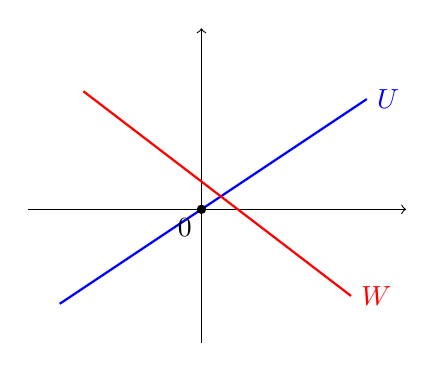
\begin{tikzpicture}[scale=1.0]
  \draw[->] (-2.2,0)--(2.6,0);
  \draw[->] (0,-1.7)--(0,2.3);
  \draw[thick,blue] (-1.8,-1.2)--(2.1,1.4) node[right] {$U$};
  \draw[thick,red] (-1.5,1.5)--(1.9,-1.1) node[right] {$W$};
  \fill (0,0) circle (1.7pt) node[below left] {$0$};
\end{tikzpicture}
\end{center}

上图表示 $\R^2$ 中两条过原点而方向不同的直线。它们的交只有零向量，且和空间为整个 $\R^2$，因此 $\R^2=U\oplus W$。

\begin{theorem}[维数公式]
设 $V$ 是有限维向量空间，$U,W$ 是 $V$ 的子空间。则
\[
\dim(U+W)=\dim U+\dim W-\dim(U\cap W).
\]
\end{theorem}

\begin{proof}
设 $\{x_1,\dots,x_r\}$ 是 $U\cap W$ 的一组基。将它扩充为 $U$ 的一组基：
\[
\{x_1,\dots,x_r,u_1,\dots,u_p\},
\]
再扩充为 $W$ 的一组基：
\[
\{x_1,\dots,x_r,w_1,\dots,w_q\}.
\]
于是
\[
\dim U=r+p,\qquad \dim W=r+q.
\]

我们证明向量组
\[
\mathcal B=\{x_1,\dots,x_r,u_1,\dots,u_p,w_1,\dots,w_q\}
\]
是 $U+W$ 的一组基。

先证张成。任取 $v\in U+W$，则 $v=u+w$，其中 $u\in U$，$w\in W$。由于上述两组分别是 $U$ 与 $W$ 的基，可写成
\[
u=\sum_{i=1}^r a_i x_i+\sum_{j=1}^p b_j u_j,
\qquad
w=\sum_{i=1}^r c_i x_i+\sum_{k=1}^q d_k w_k.
\]
相加得
\[
v=\sum_{i=1}^r (a_i+c_i)x_i+\sum_{j=1}^p b_j u_j+\sum_{k=1}^q d_k w_k,
\]
所以 $\mathcal B$ 张成 $U+W$。

再证线性无关。设
\[
\sum_{i=1}^r \alpha_i x_i+\sum_{j=1}^p \beta_j u_j+\sum_{k=1}^q \gamma_k w_k=0.
\]
移项得
\[
\sum_{i=1}^r \alpha_i x_i+\sum_{j=1}^p \beta_j u_j
=
-\sum_{k=1}^q \gamma_k w_k.
\]
左边属于 $U$，右边属于 $W$，所以它们都属于 $U\cap W$。因此左边可由 $x_1,\dots,x_r$ 线性表示。由
\[
\{x_1,\dots,x_r,u_1,\dots,u_p\}
\]
是 $U$ 的基可知 $\beta_1=\cdots=\beta_p=0$。同理，由
\[
\{x_1,\dots,x_r,w_1,\dots,w_q\}
\]
是 $W$ 的基可知 $\gamma_1=\cdots=\gamma_q=0$。最后由 $x_1,\dots,x_r$ 线性无关得 $\alpha_1=\cdots=\alpha_r=0$。故 $\mathcal B$ 线性无关。

因此 $\mathcal B$ 是 $U+W$ 的一组基，从而
\[
\dim(U+W)=r+p+q=(r+p)+(r+q)-r=\dim U+\dim W-\dim(U\cap W).
\]
\end{proof}

\begin{example}[对称矩阵与斜对称矩阵]
设 $\Char(\F)\ne 2$。记
\[
\mathrm{Sym}_n(\F)=\{A\in\Mat_n(\F):A^T=A\},
\]
\[
\mathrm{Skew}_n(\F)=\{A\in\Mat_n(\F):A^T=-A\}.
\]
则它们都是 $\Mat_n(\F)$ 的子空间，而且
\[
\Mat_n(\F)=\mathrm{Sym}_n(\F)\oplus \mathrm{Skew}_n(\F).
\]
事实上，对任意矩阵 $A$，有分解
\[
A=\frac{A+A^T}{2}+\frac{A-A^T}{2}.
\]
第一项对称，第二项斜对称。若某矩阵同时对称又斜对称，则 $A=A^T=-A^T$，故 $2A=0$。由于 $\Char(\F)\ne 2$，得 $A=0$，所以交只含零矩阵。
\end{example}

\section{商空间}

商空间的思想是：既然子空间 $U$ 内的变化“我们不想区分”，那就把只相差一个 $U$ 中向量的两个向量视为等价。

\begin{definition}
设 $U$ 是向量空间 $V$ 的子空间。在 $V$ 上定义关系
\[
v\sim w \iff v-w\in U.
\]
称其为\emph{模 $U$ 的等价关系}。$v$ 的等价类记为
\[
v+U=\{v+u:u\in U\},
\]
称为以 $v$ 为代表元的\emph{陪集}（或\emph{仿射陪集}）。所有这类等价类构成的集合记为 $V/U$。
\end{definition}

\begin{proposition}
上述关系 $\sim$ 是一个等价关系。
\end{proposition}

\begin{proof}
自反性：对任意 $v\in V$，有 $v-v=0\in U$，故 $v\sim v$。

对称性：若 $v\sim w$，则 $v-w\in U$。由于 $U$ 是子空间，所以 $-(v-w)=w-v\in U$，因此 $w\sim v$。

传递性：若 $v\sim w$ 且 $w\sim z$，则 $v-w\in U$ 且 $w-z\in U$。由子空间对加法封闭得
\[
(v-w)+(w-z)=v-z\in U,
\]
故 $v\sim z$。
\end{proof}

\begin{proposition}[商空间运算的良定义]
在 $V/U$ 上定义
\[
(v+U)+(w+U)=(v+w)+U,
\]
\[
a(v+U)=(av)+U\qquad (a\in\F).
\]
则这些定义与代表元的选择无关，从而使 $V/U$ 成为 $\F$ 上的向量空间。
\end{proposition}

\begin{proof}
先证加法的良定义。若 $v+U=v'+U$ 且 $w+U=w'+U$，则 $v-v'\in U$、$w-w'\in U$。因此
\[
(v+w)-(v'+w')=(v-v')+(w-w')\in U,
\]
所以 $(v+w)+U=(v'+w')+U$。

再证数乘的良定义。若 $v+U=v'+U$，则 $v-v'\in U$。由于 $U$ 对数乘封闭，
\[
a(v-v')=av-av'\in U,
\]
故 $(av)+U=(av')+U$。

现在验证向量空间公理。它们都可从 $V$ 中相应的公理直接推出。例如
\[
((v+U)+(w+U))+(z+U)=((v+w)+z)+U=(v+(w+z))+U,
\]
所以加法结合律成立；零元是 $U=0+U$；$v+U$ 的加法逆元是 $(-v)+U$；其余公理完全类似。因此 $V/U$ 是向量空间。
\end{proof}

\begin{example}[平面模掉一条直线]
令 $V=\R^2$，$U=\{(x,0):x\in\R\}$ 为 $x$ 轴。则
\[
(a,b)+U=\{(a+t,b):t\in\R\}
\]
是平面中与 $x$ 轴平行的一条水平直线。两个点属于同一陪集，当且仅当它们具有相同的第二坐标。因此 $V/U$ 中每个元素都由一个实数 $b$ 唯一标记；直观上说，商空间把“沿着 $x$ 轴的方向”压缩掉了。
\end{example}

\begin{theorem}[自然投影]
映射
\[
\pi:V\to V/U,\qquad \pi(v)=v+U,
\]
称为从 $V$ 到 $V/U$ 的\emph{自然投影}。它满足：
\begin{enumerate}[label=\textnormal{(\arabic*)}]
  \item $\pi(v+w)=\pi(v)+\pi(w)$；
  \item $\pi(av)=a\pi(v)$；
  \item $\pi(v)=U$ 当且仅当 $v\in U$；
  \item 每个陪集都形如 $\pi(v)$，因此 $\pi$ 是满的。
\end{enumerate}
\end{theorem}

\begin{proof}
前两条直接由商空间中的运算定义得到：
\[
\pi(v+w)=(v+w)+U=(v+U)+(w+U)=\pi(v)+\pi(w),
\]
\[
\pi(av)=av+U=a(v+U)=a\pi(v).
\]

对于 (3)，有
\[
\pi(v)=U\iff v+U=0+U\iff v-0\in U\iff v\in U.
\]

对于 (4)，$V/U$ 的元素按定义就是各个陪集，而每个陪集都可写成 $v+U=\pi(v)$，所以 $\pi$ 的像就是整个 $V/U$。
\end{proof}

\begin{theorem}[商空间的维数公式]
设 $V$ 是有限维向量空间，$U$ 是其子空间。则
\[
\dim(V/U)=\dim V-\dim U.
\]
\end{theorem}

\begin{proof}
设 $\{u_1,\dots,u_r\}$ 是 $U$ 的一组基，并将它扩充为 $V$ 的一组基：
\[
\{u_1,\dots,u_r,v_1,\dots,v_s\}.
\]
于是
\[
\dim U=r,\qquad \dim V=r+s.
\]

我们证明
\[
\{v_1+U,\dots,v_s+U\}
\]
是商空间 $V/U$ 的一组基。

先证张成。任取 $x+U\in V/U$。因为上面的向量组是 $V$ 的基，存在唯一的标量 $a_1,\dots,a_r,b_1,\dots,b_s$ 使得
\[
x=a_1u_1+\cdots+a_ru_r+b_1v_1+\cdots+b_sv_s.
\]
把属于 $U$ 的部分并入陪集即可得
\[
x+U=b_1(v_1+U)+\cdots+b_s(v_s+U).
\]
所以这些陪集张成 $V/U$。

再证线性无关。若
\[
b_1(v_1+U)+\cdots+b_s(v_s+U)=U,
\]
则
\[
(b_1v_1+\cdots+b_sv_s)+U=U,
\]
故 $b_1v_1+\cdots+b_sv_s\in U$。于是存在标量 $a_1,\dots,a_r$ 使得
\[
b_1v_1+\cdots+b_sv_s=a_1u_1+\cdots+a_ru_r.
\]
移项得到
\[
a_1u_1+\cdots+a_ru_r-b_1v_1-\cdots-b_sv_s=0.
\]
由于
\[
\{u_1,\dots,u_r,v_1,\dots,v_s\}
\]
是 $V$ 的基，故它线性无关，从而 $b_1=\cdots=b_s=0$。因此 $v_1+U,\dots,v_s+U$ 线性无关。

综上，$\{v_1+U,\dots,v_s+U\}$ 是 $V/U$ 的一组基，故
\[
\dim(V/U)=s=(r+s)-r=\dim V-\dim U.
\]
\end{proof}

\begin{example}[多项式空间的商]
取 $V=\R[x]_{\le 3}$，$U=\R[x]_{\le 1}$。则
\[
\dim V=4,\qquad \dim U=2,
\]
所以 $\dim(V/U)=2$。事实上，$x^2+U$ 与 $x^3+U$ 构成 $V/U$ 的一组基，因为任意三次以下多项式在模掉常数项与一次项后，只剩下二次项和三次项的信息。
\end{example}

\begin{remark}[与模形式空间的联系]
以后我们会遇到复向量空间 $M_k(\Gamma)$，它由某个群 $\Gamma$ 的权 $k$ 模形式组成。子空间 $S_k(\Gamma)$ 由尖点模形式组成；此时商空间 $M_k(\Gamma)/S_k(\Gamma)$ 可以理解为“把尖点部分视为零以后剩下的 Eisenstein 部分”。即使暂时不了解模形式，读者也应当熟悉这种“模掉一个已知子空间”的思想。
\end{remark}

\section*{习题}

下面共有 $60$ 道习题，分为基础、进阶、挑战三级。建议先独立完成基础题，再系统练习进阶题，最后尝试挑战题。

\subsection*{基础题}
\begin{enumerate}[label=\arabic*., leftmargin=2.5em]
  \item \basic 验证 $\R^n$ 在按分量加法与按分量数乘下满足向量空间的八条公理。
  \item \basic 说明 $\C^n$ 既可以看成 $\C$ 上的向量空间，也可以看成 $\R$ 上的向量空间。两种看法下的标量分别是什么？
  \item \basic 证明 $\R^2$ 中的集合 $U=\{(x,2x):x\in\R\}$ 是子空间，并求它的一组基。
  \item \basic 判断集合 $S=\{(x,y)\in\R^2:x+y=1\}$ 是否是 $\R^2$ 的子空间，并说明理由。
  \item \basic 证明 $\F[x]_{\le 3}$ 是 $\F[x]$ 的子空间，并写出它的一组基。
  \item \basic 判断 $\F[x]$ 中所有非零多项式组成的集合是否是子空间，并说明理由。
  \item \basic 求解方程 $x+y+z=0$ 在 $\R^3$ 中的解空间，并给出一组基。
  \item \basic 判断向量 $(1,0,1),(0,1,1),(1,1,2)$ 在 $\R^3$ 中是线性相关还是线性无关。
  \item \basic 判断多项式 $1+x,\ x+x^2,\ 1+2x+x^2$ 是否线性无关。
  \item \basic 证明函数 $\sin x$ 与 $\cos x$ 在实向量空间 $\R^{\R}$ 中线性无关。
  \item \basic 证明：任何含零向量的有限向量组都线性相关。
  \item \basic 证明：若 $v\ne 0$ 且 $w=av$，则 $\{v,w\}$ 线性相关。
  \item \basic 从向量组
  \[
  (1,0,0),(0,1,0),(1,1,0),(0,0,1)
  \]
  中找出一个极大的线性无关子集。
  \item \basic 求 $\R^4$ 中向量组
  \[
  (1,0,1,0),(0,1,0,1),(1,1,1,1)
  \]
  的张成空间的一组基。
  \item \basic 在基 $\mathcal B=\{(1,0),(1,1)\}$ 下求向量 $(3,5)$ 的坐标。
  \item \basic 在基 $\mathcal B=\{1,x,x^2\}$ 下求多项式 $2-3x+x^2$ 的坐标。
  \item \basic 设 $\mathcal B=\{(1,0),(1,1)\}$，$\mathcal C=\{(1,1),(0,1)\}$。求 $(2,1)$ 在这两组基下的坐标。
  \item \basic 证明：两个子空间的交仍是子空间。
  \item \basic 在 $\R^2$ 中取
  \[
  U=\{(x,0):x\in\R\},\qquad W=\{(x,x):x\in\R\}.
  \]
  求 $U+W$。
  \item \basic 判断上题中的 $\R^2$ 是否等于 $U\oplus W$。
  \item \basic 设 $U,W\subseteq \R^4$ 是子空间，且 $\dim U=2,\dim W=3,\dim(U\cap W)=1$。求 $\dim(U+W)$。
  \item \basic 写出一维向量空间 $V$ 的全部子空间。
  \item \basic 证明 $\Mat_2(\R)$ 中全体对角矩阵构成子空间，并求其一组基。
  \item \basic 求 $\mathrm{Sym}_2(\R)$ 的一组基。
  \item \basic 求 $\mathrm{Skew}_3(\R)$ 的一组基。
  \item \basic 在 $V=\R^2$、$U=\{(x,0):x\in\R\}$ 的情形下，描述陪集 $(a,b)+U$ 的几何形状。
  \item \basic 设 $U=\mathrm{span}\{(1,0,0),(0,1,0)\}\subseteq \R^3$。求 $\dim(\R^3/U)$。
  \item \basic 设 $\pi:V\to V/U$ 是自然投影。证明 $\pi(v)=U$ 当且仅当 $v\in U$。
  \item \basic 说明为什么齐次线性方程组的解集是子空间，而非齐次线性方程组的解集一般不是子空间。
  \item \basic 说明常数函数全体构成一个复向量空间，并给出其维数。
\end{enumerate}

\subsection*{进阶题}
\begin{enumerate}[label=\arabic*., start=31, leftmargin=2.5em]
  \item \medium 证明：有限张成组中的极大线性无关子集一定是一组基。
  \item \medium 证明：若一个有限向量组张成某空间且删去其中任一向量后都不再张成该空间，则该向量组线性无关。
  \item \medium 设 $v_1,\dots,v_r$ 线性相关。证明：存在某个指标 $k$，使得 $v_k\in \mathrm{span}(v_1,\dots,v_{k-1})$。
  \item \medium 将线性无关组 $\{1,x^2\}$ 扩充为 $\R[x]_{\le 4}$ 的一组基。
  \item \medium 设 $U=\mathrm{span}\{(1,1,0,0),(0,0,1,1)\}\subseteq \R^4$。构造 $\R^4$ 的一组基，其前两个向量恰好构成 $U$ 的一组基。
  \item \medium 证明：有限维向量空间的任意子空间仍为有限维。
  \item \medium 设 $U,W$ 是有限维向量空间 $V$ 的子空间，且 $\dim U+\dim W>\dim V$。证明 $U\cap W\ne \{0\}$。
  \item \medium 设 $U,W\subseteq V$，且 $\dim U+\dim W=\dim V$ 并满足 $U\cap W=\{0\}$。证明 $V=U\oplus W$。
  \item \medium 设 $\Char(\F)\ne 2$。证明任意 $A\in \Mat_2(\F)$ 都能唯一写成一个对称矩阵与一个斜对称矩阵之和。
  \item \medium 设 $\Char(\F)\ne 2$。证明
  \[
  \Mat_n(\F)=\mathrm{Sym}_n(\F)\oplus \mathrm{Skew}_n(\F),
  \]
  并求这两个子空间的维数。
  \item \medium 设 $E\subseteq \R[x]_{\le n}$ 为偶多项式空间，$O\subseteq \R[x]_{\le n}$ 为奇多项式空间。证明
  \[
  \R[x]_{\le n}=E\oplus O.
  \]
  \item \medium 求子空间
  \[
  U=\{(x_1,\dots,x_n)\in \F^n:x_1+\cdots+x_n=0\}
  \]
  的一组基，并求其维数。
  \item \medium 设 $U=\mathrm{span}\{e_1,e_2\}$，$W=\mathrm{span}\{e_3,e_4,e_5\}$，其中 $e_i$ 是 $\R^5$ 的标准基。证明 $\R^5=U\oplus W$。
  \item \medium 设 $V=\F[x]_{\le 5}$，$U=\F[x]_{\le 2}$。写出 $V/U$ 的一组基并求其维数。
  \item \medium 证明：$V/U$ 一维当且仅当 $U$ 是 $V$ 的真子空间且 $\dim U=\dim V-1$。
  \item \medium 完整证明商空间加法与数乘的定义与代表元无关。
  \item \medium 设 $V=U\oplus W$。证明每个陪集 $v+U$ 都含有唯一一个来自 $W$ 的向量。由此说明 $V/U$ 与 $W$ 在向量空间意义下“本质相同”。
  \item \medium 设 $\{u_1,\dots,u_r,v_1,\dots,v_s\}$ 是 $V$ 的一组基，其中 $\{u_1,\dots,u_r\}$ 是子空间 $U$ 的一组基。证明 $\{v_1+U,\dots,v_s+U\}$ 是 $V/U$ 的一组基。
  \item \medium 已知对某个群 $\Gamma$ 和偶整数 $k\ge 4$，有
  \[
  M_k(\Gamma)=S_k(\Gamma)\oplus \C E_k,
  \]
  其中 $E_k$ 是一个固定的 Eisenstein 级数。证明
  \[
  \dim M_k(\Gamma)=\dim S_k(\Gamma)+1.
  \]
  \item \medium 用“先取 $U\cap W$ 的基并分别扩充”的方法，重新证明维数公式
  \[
  \dim(U+W)=\dim U+\dim W-\dim(U\cap W).
  \]
\end{enumerate}

\subsection*{挑战题}
\begin{enumerate}[label=\arabic*., start=51, leftmargin=2.5em]
  \item \hard 证明多项式空间 $\F[x]$ 不是有限维向量空间。
  \item \hard 设 $V$ 是所有仅有有限多个非零项的数列
  \[
  (a_0,a_1,a_2,\dots)
  \]
  的集合。证明 $V$ 是向量空间，并找出它的一组可数基。
  \item \hard 设 $a_1,\dots,a_r\in\R$ 两两不同。证明函数 $e^{a_1x},\dots,e^{a_rx}$ 在线性空间 $\R^{\R}$ 中线性无关。
  \item \hard 设 $V$ 是无限维向量空间。证明：不存在有限子集能够张成整个 $V$。
  \item \hard 设 $\F$ 是无限域，$V$ 是有限维非零向量空间。证明：有限个真子空间的并不可能等于 $V$。
  \item \hard 设 $V=\F[x]$，$U=x\F[x]=\{xf(x):f(x)\in\F[x]\}$。证明 $V/U$ 是一维向量空间。
  \item \hard 假设已知分次环恒等式
  \[
  M_*(\SL_2(\Z))=\C[E_4,E_6].
  \]
  证明对每个偶整数 $k\ge 0$，$M_k(\SL_2(\Z))$ 的维数等于满足 $4a+6b=k$ 的非负整数解 $(a,b)$ 的个数。
  \item \hard 在上题假设下，再假设对偶整数 $k\ge 4$ 有分解
  \[
  M_k(\SL_2(\Z))=S_k(\SL_2(\Z))\oplus \C E_k.
  \]
  证明
  \[
  \dim S_k(\SL_2(\Z))=\dim M_k(\SL_2(\Z))-1.
  \]
  \item \hard 证明多项式空间 $\F[x]$ 可写成偶多项式子空间与奇多项式子空间的直和。
  \item \hard 设 $V$ 是所有从 $\N$ 到 $\F$ 的函数组成的空间。证明其中的多项式函数集合构成 $V$ 的一个真子空间，并说明该子空间仍是无限维的。
\end{enumerate}

